\documentclass[a4paper,12pt,oneside]{report}
\usepackage[T1]{fontenc}
\usepackage{setspace}
\usepackage[utf8]{inputenc} 
\usepackage[english]{babel}
\usepackage{url}
\usepackage{ctable}
\usepackage{layaureo}
\usepackage[english]{varioref}
\usepackage{mathtools}
\usepackage{siunitx}
\usepackage{amsfonts}
\usepackage{amsmath}
\usepackage{microtype}
\usepackage{booktabs}
\usepackage[font=small,labelfont=bf]{caption}
\usepackage{subfig}
\usepackage{appendix}
\usepackage{fancyhdr}
\usepackage{graphicx}
\usepackage{xcolor}
\usepackage[autostyle,italian=guillemets]{csquotes}
\usepackage{listings,xcolor}
\pagestyle{fancy}
\fancyhf{}
\fancyhead[R]{\thepage}
\renewcommand{\chaptermark}[1]{\markboth{#1}{#1}}
\fancyhead[L]{\scshape{\chaptername} \thechapter\ --\ \leftmark}
\newlength{\mylen}
\setbox1=\hbox{$\bullet$}\setbox2=\hbox{\tiny$\bullet$}
\setlength{\mylen}{\dimexpr0.5\ht1-0.5\ht2}
\renewcommand\labelitemi{\raisebox{\mylen}{\tiny$\bullet$}}
\onehalfspacing
%\usepackage[backend=biber,style=numeric-comp]{biblatex}
\DeclarePairedDelimiter{\abs}{\lvert}{\rvert}
\DeclarePairedDelimiter{\norma}{\lVert}{\rVert}
%\addbibresource{Bibliografia.bib}
\graphicspath{{./Images/}}
\usepackage{hyperref}
\hypersetup{hidelinks}
%\pagestyle{headings}
\newcommand{\Hline}{\specialrule{.1em}{0em}{0em}}
\begin{document}
\begin{titlepage}

\begin{figure}
\centering

\includegraphics[scale=0.25]{sigillo2}
\end{figure}

\begin{center}
\LARGE{\textbf{Università degli Studi di Trento\\ Department of Industrial Engineering}}\\
\vspace{10mm}
\Large{Master Degree in\\ Mechatronics Engineering}\\
\vspace{7mm}
\uppercase{Final Dissertation}
\vspace{7mm}\\
\huge{Titolo}
\end{center}

\vspace{8mm}
\begin{flushleft}
\large{\textbf{Supervisor:}\\ Daniele Bortoluzzi}\\
\vspace{5mm}
\large{\textbf{Co-supervisor:}\\ Edoardo Dalla Ricca}\\
\vspace{5mm}
\large{\textbf{Student:}\\ Simone Manfredi 239337}\\
\end{flushleft}

\vspace{15mm}
\begin{center}
\Large{Academic Year 2023/2024}
\end{center}

\end{titlepage}

\newpage

\begin{abstract}


\end{abstract}

\newpage

\pagenumbering{roman}
\addcontentsline{toc}{chapter}{Contents}

\tableofcontents

\chapter*{Introduction}
\addcontentsline{toc}{chapter}{Introduction}
We live in a society overwhelmed by such technology, autonomous systems, industrial manipulators, AI and, very soon, services' humanoid robots, that we forget to look up in the sky. Most of the major progress in robotics and the scientific field is done in space, where human curiosity is pushing our abilities beyond any imaginable scenario.\\
This thesis was born due to my curiosity in the field of robotics merged with the need to face space and modern problems, such as the berthing and docking of external objects by a manipulator or the tumbling of a spinning satellite. This dissertation aims to analyse the dynamic of a space manipulator after the impact with an external satellite/meteorite to retrieve its kinetic properties before the impact.\\
\clearpage
\pagenumbering{arabic}
\chapter{Space Manipulators: an Overview}
Space Robotics is important to human's overall ability to explore or operate in space. Autonomous systems can reduce the cognitive load on humans and improve human and systems' safety.\\
Space robots can be split into two main categories: orbital robots and planetary robots. The formers can be used for repairing satellites, assembling large space telescopes, capturing and returning asteroids, etc; the latter play a key role in surveying, observations, extraction, working on planetary surfaces for subsequential human arrival, etc.\\
Furthermore, spacecraft are classified as space robots when two attributes are satisfied: locomotion and autonomy. Depending on its application, a space robot is designed to possess locomotion to manipulate, grip, rove, drill and/or sample; at the same time, it is expected to possess varying levels of autonomy, ranging from teleoperation by humans to fully autonomous operation by the robot itself [3].\\
Another classification of robotic devices in space could be represented by mobile robots, flying robots, and manipulators. Manipulators are used on board spacecraft (Space Shuttle) or space stations [5].
According to [1], a very loose definition calls every unmanned space probe a robotic spacecraft, referring to the challenges of largely autonomous operation in a complex mission. But even discarding this and focussing on space robotics elements in a more narrow sense (systems involving arms for manipulation or some kind of locomotion device for mobility and having the flexibility to perform varying tasks), there is a wide array of uses in the scope of space missions, giving rise to challenging problems and ingenious solution.\\
Robots and manipulators in space are designed to perform the following operations:
\begin{itemize}
\item capture
\item maneuvring
\item berthing/unberthing
\item support of Extra-Vehicular-Activities (EVA)
\item positioning and release
\end{itemize}
One of the most important features of all robots deployed in space is their flexibility. Robots and manipulators used in space are built out of light materials, and very often, their links deflect.\\
There are quite a number of on-orbit applications requiring advanced robotics capabilities, which
are envisaged to take place in the 2025-2035 timeframe. The operators for these missions may
range from space administrations to national governments to businesses. The following mission
foci are envisaged: space debris removal, rescue mission, planned orbit raising,
inspection/support to deployment, deployment/assembly aid, repair, refuelling and orbit
maintenance, mission evolution/adaptation, lifetime extension, and re/de-orbiting. The
International Space Station (ISS) continues to represent an excellent opportunity for scientific
experiments to be conducted in space amid the unique characteristics, constraints and pressures that the environment brings [3].\\
But what is so special about a space robot? In many ways, robot systems for space applications are very different from the more familiar terrestrial robots, be they industrial robots in production automation or the newer kind of "service robots". One of the main and simplest differences is the high development and manufacturing costs and the missing "economy of scale" due to the experimental prototype nature of these developments.\\
This thesis will investigate space manipulators' dynamics, whose tasks involve berthing and docking satellites or managing tumbling meteorites; thus, a historical summary of their evolution and the actual state-of-art of this field will be briefly exposed.
\newpage
\section{Historical background}
The first robot used in space was the Remote Manipulator System (RMS), also called \textit{Canadarm}, developed by the Canadian Space Agency and mounted on the Space Shuttle. This robot was used for the first time on 12th November 1981 in the Columbia Shuttle and it was retired in July 2011. It is 15 meters long and has three hinged joints for pitch and three others for yaw and roll, which makes a total of six degrees of freedom (DOF).\\
There were numerous problems related to the use of the RMS in space. One of the most important was related to its positioning: since it is built out of light materials to minimise the launch cost, its links deflect substantially. When the arm is accelerated and stopped, large vibrations occur.\\
There are two main methods of improving the positioning accuracy of the RMS: passive and active. The passive methods focus on redesigning the manipulator and applying different materials. The active ones refer to a preshape input and to the usage of position, velocity or force feedback.\\
Eventually, some lessons have been learnt during the RMS' lifetime: the speed of manipulation should be drastically improved; the positioning accuracy is one of the most important issues in day-to-day operations; the new manipulators should be designed to include passive vibration control capabilities; active vibration control should be added in order to improve the positioning accuracy and shorten the settling time; the force loop could add significantly to the capabilities of the manipulator [5].\\
It is interesting to note that the actuators are not powerful enough to lift even the weight of the arm itself when on Earth. The Canadarm has been used for over 100 operations and is normally used for repairing, retrieving, and deploying satellites; assisting humans during extravehicular activi- ties; and for remote inspection tasks [6].\\
Another early mission including a robotic arm in space was the MIR space station. This Soviet Union/Russian space station was the first modular space station and was in operation from 1986 to 2001. MIR was a microgravity research laboratory which conducted research in biology, astronomy, meteorology, and physics, to name a few. Four of the modules were equipped with the Lyappa robotic arm used for assembling the modules of the space station.\\
In 1997 the National Space Development Agency of Japan (NASDA) launched the Engineering Test Satellite No. 7 (ETS-VII), the first ever satellite to be equipped with a robotic arm. The ETS-VII performed several successful docking operations using the manipulator arm. The main objectives of the project were performance evaluation of a satellite-mounted robotic system; coordinated control of the satellite attitude and robot arm; teleoperation of the robot arm; demonstration of in-orbit satellite servicing.\\
The project demonstrated the successful execution of experiments which gained insight into operations such as docking, fuel transfer, assembling, and berthing. Several successful docking operations were performed with the chaser and target satellite.\\
The Japanese also developed a robotic arm which was mounted on the Japanese Experiment Module at the International Space Station (ISS), the JEMRMS, in March 2008. The Small Fine Arm (SFA) was added in July 2009 (see Section~\ref{state_of_art}).\\
A larger and more advanced version of the SRMS arm is the MSS arm (Mobile Servicing System), which is mounted on the International Space Station. The MSS arm consists of a mobile base, a more advanced version of the Canadarm, called the \textit{Canadarm2}, or SSRMS, and dexterous manipulator hand [6]. It has seven DOF, unlike the RMS, making it a redundant manipulator to avoid singularities in some specific but important positions. Its properties will be discussed in the next Section. [5]\\
In March 2008 the last part of the Mobile Servicing System was added to the International Space Station. The Canada Hand, or the Special Purpose Dexterous Manipulator (SPDM), is a two-armed robot but is often referred to as a hand be- cause it can be attached to the Canadarm2 robotic arm and taken to any location on the space station [6].\\
The last manipulator in space was launched in July 2021: the Europian Robotic Arm (ERA) serves as main manipulator on the Russian part of the Space Station.\\
Clearly, the usage of manipulator in space involves recent activities, hence a lot of research and experiments are still in development. This research field offers numerous starting points in analysis and technologic progress.
\newpage
\section{Main characteristics}
Orbiting robotic systems consist of a free-floating base, typically a satellite or a space station, with a robotic manipulator attached to it.\\
The main difference between space manipulators and Earth-based robots is the lack of a fixed base on which the robot is mounted.\\
Depending on whether or not actuation is utilized to control the spacecraft position and orientation, we can divide these systems into \textit{free-flying} and \textit{free-floating} space manipulators. \\
In a free-flying robotic system the position and orientation of the base, in this case the spacecraft, is actively controlled by the spacecraft’s actuators. This allows to completely control both the base configuration and the manipulator arm.\\ 
Due to the dynamic coupling between the manipulator and the spacecraft, the motion of the manipulator arm will constantly affect the motion of the base. The main concern with these systems is therefore the excessive fuel consumption required to compensate for the dynamic coupling between the manipulator and the base while maintaining a constant base attitude [6].\\
This mode is employed during the final approach of a manipulator to its target, so that the target is within the manipulator workspace [2].\\
A free-floating robotic system, on the other hand, does not use spacecraft actuation to compensate for the manipulator motion. The spacecraft motion is therefore not controlled directly, but arises as a result of the dynamic coupling between the manipulator and the base. In this case one can either choose not to control the spacecraft motion at all, or to use the manipulator arm to obtain the required motion also for the spacecraft. In many cases it is necessary to generate a manipulator motion which guarantees that the spacecraft orientation remains almost constant so that antennas and other instruments point in the right direction [6].\\
In this mode, the spacecraft attitude is controlled actively with momentum control devices (MCD), such as reaction wheels or momentum gyros, while the system CoM does not translate. The free-floating or the partial free-floating modes are preferred during grasping, since they eliminate sudden motions due to thrusters, and conserve propellant and power [2].\\
Even though space exploration is challenging compared to Earth-based systems, space manipulator design also benefits from the free-fall environment in some areas. It is, for example, possible to construct robots with extremely high redundancy and with several joints. This type of robots, are able to support their own weight in space due to the small gravitational forces. On Earth, however, such robots would collapse due to their own weight when the number of joints becomes too large. This allows for more redundant robots in space than on Earth, and also more fault tolerant robots because the robots can continue operation even after several joint failures. Similarly, the free-fall environment allows for effective control with very small actuators. In fact, most space manipulators are able to handle very high payloads in space, while they cannot even withstand the weight of the manipulator arm itself if they were to be placed in the Earth’s gravity field [6].\\
\textcolor{red}{WHICH ONES ARE CONSIDERED IN THIS WORK?}\\

To execute on-orbit tasks being inaccessible to, or too dangerous for humans, robotic on-orbit servicing (OOS) can be employed, with tasks to be performed by space manipulator systems (SMSs), also called chasers or servicers in the literature. An SMS consists of a satellite base equipped with one or more robotic manipulators (arms) with grappling devices on them and driven by a vision system which allows them to capture a target (client) satellite, or another object. An SMS also can be a large servicing manipulator mounted on a space facility.\\
Targets for capture may be cooperative, i.e., a stable and safe target due to its operational Attitude and Orbit Control Subsystem (AOCS), or non-cooperative i.e., an unknown or tumbling target with a varying axis of rotation. They can also be collaborative, i.e., designed for capture or servicing, equipped with visual markers and grapple fixtures, or non-collaborative, as most of today’s satellites. In many cases in the literature, the term cooperative stands for collaborative, too.
As often revealed by ground observations, many on-orbit objects are tumbling in an uncontrolled way (non-cooperative targets), making the robotic capture a very challenging task. This is the case analysed in this thesis.\\
Clearly, only after a manipulator has successfully captured and stabilized a tumbling target, can a service operation be started. Therefore, a common robotic capture task for on-orbit servicing consists of four operational phases: 
\begin{enumerate}
  \item observation and planning phase;
  \item final approach phase;
  \item impact and grasping/capture phase;
  \item post-capture stabilization phase.
\end{enumerate}
\textcolor{red}{WHICH ONES ARE CONSIDERED IN THIS WORK?}\\
With a target locally stationary, the approach phase can be achieved by point-to-point planning and depending on the actuation mode, by simple on-off thruster control, and attitude fine-tuning using momentum exchange devices. Capturing a tumbling, non-cooperative target is more challenging, as here velocity matching between the SMS end-effector and the capture point is required.\\
In fact, to avoid impacts during the grasping phase, the difference between the velocities of the target and the end-effector should be zero. In practise, this never happens, thus small impacts and vibrations have to be taken into account. Research on this topic is still going on, some focusing on bio-inspired isolation systems ([2018], [2020]).\\
In deploying a SMS for target capture, a manipulator trajectory is needed to achieve the goal. Several secondary optimization goals, such as obstacle and singularities avoidance, fuel consumption, and base disturbance minimization [1999] can be sought, too. E.g. [2009] focuses on the optimal time needed to reach the target [2].
\newpage
\section{State-of-art}\label{state_of_art}
The Low Earth Orbit (LEO), a whole band of orbits between 300 and 700 km altitude, is the main of today's manned space missions. This class belongs to the US Skylab, the Space Shuttle, the Russian Space Station Mir, and the International Space Station (ISS). The orbits are just high enough to be practically free of destabilising dynamic disturbances but as low as possible to minimise launch costs.\\
Apart from human physiology interest (to investigate the effects of weightlessness on astronauts), the main application field has always been a microgravity research. The term "microgravity" refers to the typical level of "weightlessness" on such manned missions: due to various disturbances (remaining atmospheric drag, moving machinery, but most of all man motion), some 10e-6 g acceleration will continue to act on every mass [1].\\
Nowadays, as already mentioned, on the ISS there are three main SMSs:
\begin{enumerate}
  \item SSRMS: Space Station Remote Manipulator System
  \item SPDM: Special Purpose Dexterous Manipulator
  \item JEMRMS: Japanese Experiment Module Remote Manipulator System
  \item ERA: European Robotic Arm
\end{enumerate}
The ISS assembly, maintenance and scientific research tasks depend on the three robotic manipulators carrying out their intended operations. Each manipulator has a specific purpose and each has been designed to successfully complete its assigned mission.\\
All three ISS robotic manipulators are designed to resemble the human arm. They are mechanically and electrically connected to the ISS at the shoulder, which is comprised of a set of revolute mechanical joints. A boom segment and then an elbow joint follow the shoulder. After the elbow there is another boom segment followed by a set of wrist joints and an end effector through which the operational grappling is carried out.[2]
\subsection{SSRMS}
The SSRMS, or Canadarm2, is primarily used for ISS assembly. This involves acquiring an assembly payload, either directly from the Shuttle Payload Bay or handed off from the Shuttle Remote Manipulator System (SRMS). The SSRMS is also used to manoeuvre astronauts and whatever they are holding from point to point as they complete their tasks during the EVA.\\
The 16.9m SSRMS has 7 offset joints and is symmetric about the elbow with identical 3DOF shoulder and wrist clusters (Figure \ref{SSRMS_dim}). The shoulder/wrist clusters contain three mechanical joints with perpendicular rotation axes: pitch, yaw and roll. One joint cluster acts as the shoulder while the other acts as the wrist of the manipulator. All of the SSRMS joints are functionally identical with the same performance capabilities and angular range of $\pm 270$ degrees. \\
The three pitch and two roll joints are identical and interchangeable. The two yaw joints are identical and interchangeable (the difference between the yaw and pitch/roll joints being that the yaw joints have a 5.25 inch extension non one end). Each of the joints is an ORU and each contains two identical joint electronics units and motor modules.\\
Attached to the roll joint on each cluster is a Latching End Effector (LEE) which provides a mechanical and electrical connection to a payload, SPDM or the ISS when grappling an SSRMS grapple fixture. In this way, it is possible for the robotic arm to move around the station's exterior. Each LEE also includes a Force Moment Sensor (FMS) and two identical LEE Electronics Units (LEUs). This symmetric configuration allows either end of the SSRMS to be attached to a Power and Data Grapple Fixture (PDGF) and to function as the base of the arm.\\
\begin{figure}[t]
  \centering
  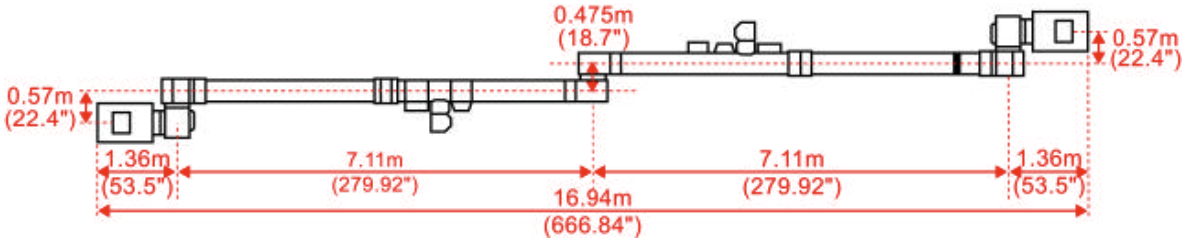
\includegraphics[scale=0.3]{SSRMS_dimensions.png}
  \caption{SSRMS Dimensions [4].}
  \label{SSRMS_dim}
\end{figure}
\begin{figure}[h]
  \centering
  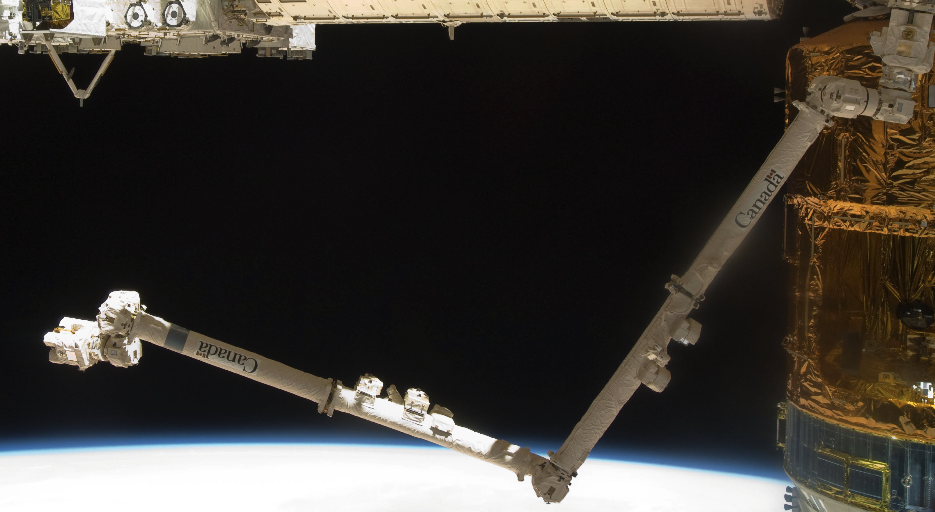
\includegraphics[scale=0.4]{SSRMS_orbit.png}
  \caption{The SSRMS on orbit [7].}
  \label{SSRMS_orbit}
\end{figure}
\subsection{SPDM}
The SPD is a highly dexterous dual-armed robot, with two shoulders that provide support for the arms.\\
Each arm has seven joints, terminating with an Orbit Replacement Unit/Tool Changeout Mechanism (OTCM), the mechanism through which the SPDM arm interfaces with payloads and tools. The SPDM is also equipped with lights, video equipment, a tool platform and four tool holders.\\
The SPDM's primary role is to carry out delicate maintenance and servicing tasks on the International Space Station. Tasks include installing and removing small payloads such as batteries, power supplies and computers; operate robotic tools such as specialized wrenches and socket extensions; provide power and data connectivity to payloads; manipulate, install, remove and inspect scientific payloads.\\
It works near the Canadarm2 and can be grapped by it to be moved around.\\
\begin{figure}[h]
  \centering
  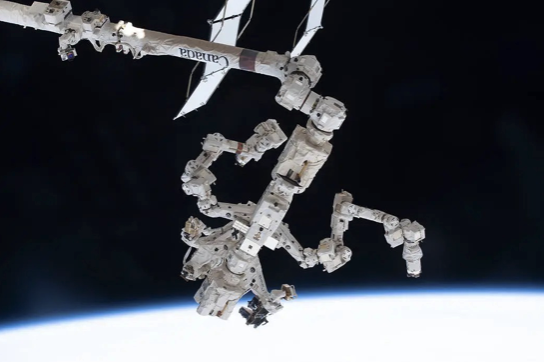
\includegraphics[scale=0.6]{SPDM.png}
  \caption{The SPDM on orbit.}
  \label{SPDM_orbit}
\end{figure}
\subsection{JEMRMS}
The JEMRMS system is used primarily for experiment payload handling. It consists of three major subsystems, the
Console, Main Arm (MA), and Small Fine Arm (SFA).\\
The Main Arm (MA) is a 10m, six-degree-of-freedom robot arm. It consists of three booms, six joints, an end effector on the tip, and two vision systems (one on the shoulder, the other on the tip).\\
The Small Fine Arm (SFA) is also asix-degree-of-freedom robot arm. It can perform more dexterous tasks than the MA. During operation, the SFA is grappled by the MA and receives power and data from the MA. The 2m SFA consists of two booms, six joints, and an end effector on the tip called the “tool,” and a camera on the tool. The tool has a force and torque sensor inside it for compliance operation [8].\\
\begin{figure}[h]
  \centering
  \subfloat[][\emph{Main Arm (MA).}]
  {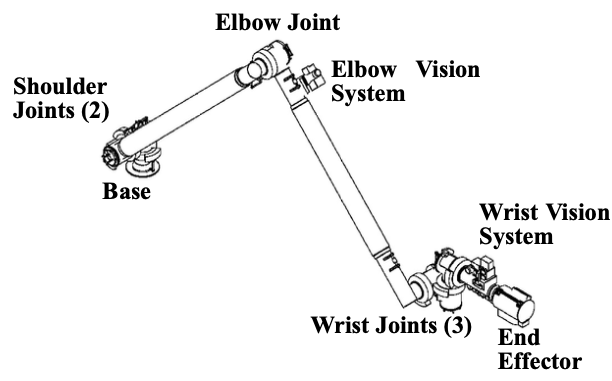
\includegraphics[scale=0.35]{MA.png}\label{unitary}} \quad
\subfloat[][\emph{Small Fine Arm (SFA).}]
  {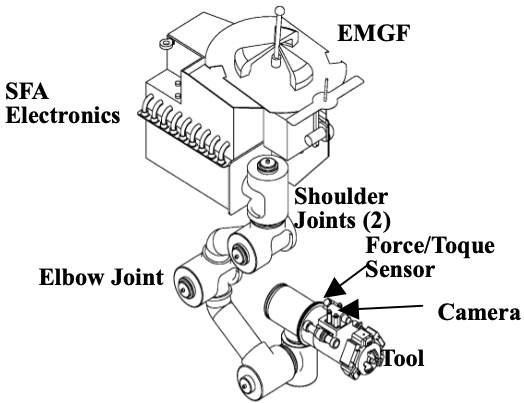
\includegraphics[scale=0.35]{SFA.png}\label{normal}} 
  \caption{The JEMRMS components. [8]}
  \label{JEMRMS_components}
\end{figure}
The JEM RMS end effector was designed based on the Shuttle RMS (SRMS) end effector. The grapple fixtures compatible with the JEMRMS MA can also be grappled by the SSRMS [4].\\
\subsection{ERA}
The ERA is used on the Russian segment (RS) of the ISS. Specific tasks for the ERA include: installing, removing or replacing experiment payloads
and large Station elements; transferring small payloads in and out of the Station through the Russian airlock; transporting crew members from one external working site
to another; freeing cosmonauts to do other work during spacewalks; using its cameras to inspect the outside of the Space Station.
The ERA manipulator arm spans 11.3m and has 7 inline joints in a symmetric configuration with respect to the elbowjoint (Figure 2). It has a shoulder with 3 DOFs, an elbow with 1 DOF and a wrist with 3 DOFs. Both the shoulder andwrist contain three functionally identical joints with mutually perpendicular rotation axes.\\
The ERA has two end effectors (EE) which can act as a base, enabling either end of the ERA to be used as the shoulder. Thus the wrist and shoulder are operationally interchangeable, just as in the SSRMS design. The identical EE’s are able to grapple and ungrapple an ERA grapple fixture, transferring power or data to an external device/load. The EE also has an Integrated Service Tool (IST) which is a built-in motorized "screwdriver" that can provide mechanical torque
actuation.\\
The ERA is equipped with four Camera and Lighting Units (CLU) one on each EE and one on either side of the elbow. The CLU will be used to provide video images of operational tasks and, if necessary, to illuminate the scene and to act as an optical sensor to enable proximity control of a target during approach of a basepoint or grapple fixture in closed loop. The proximity control function enables ERA to approach grapple fixtures automatically and smoothly [4].
\begin{figure}[h]
  \centering
  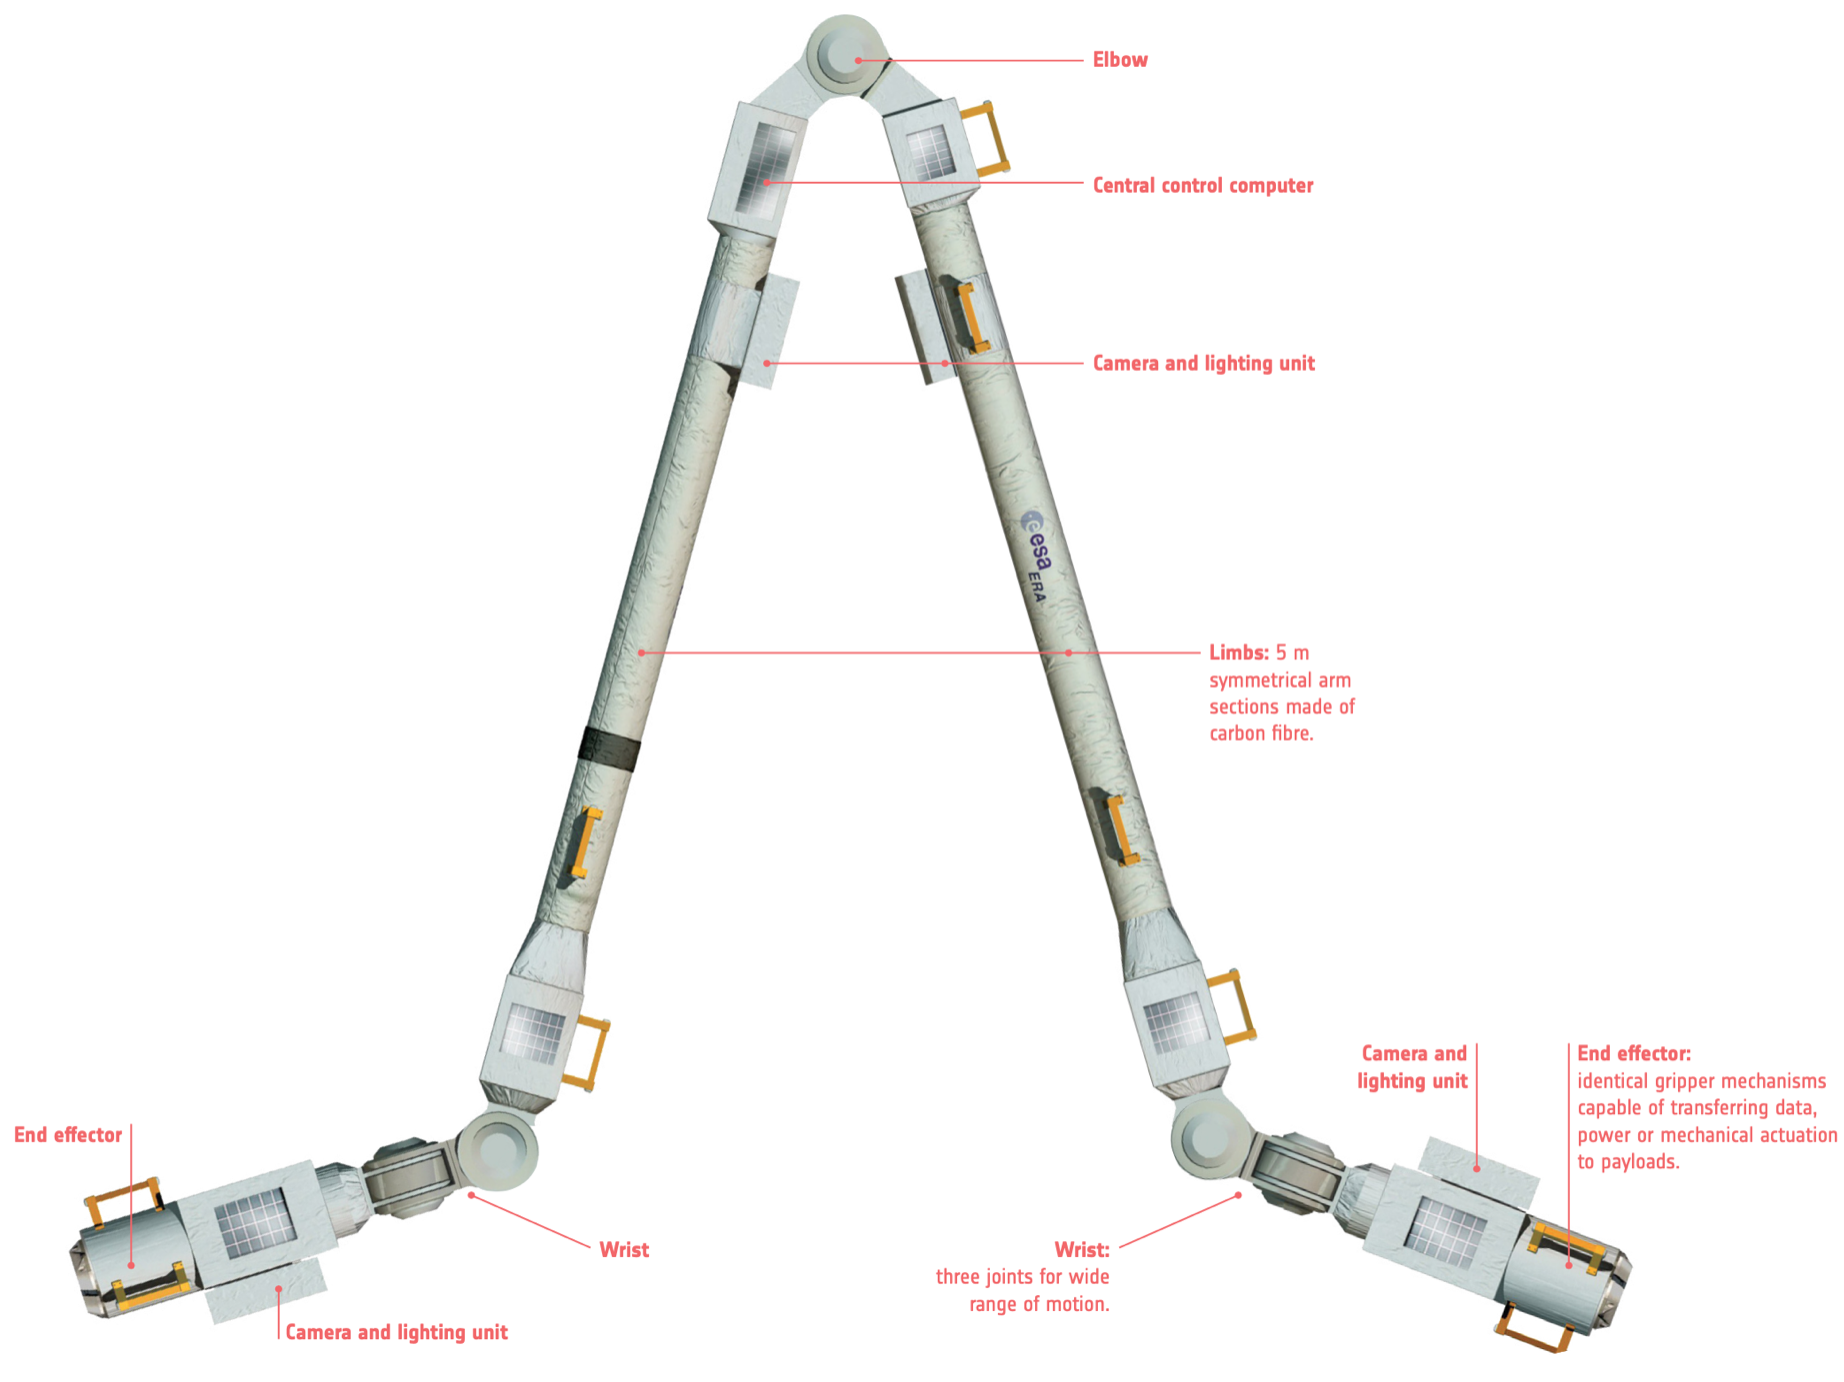
\includegraphics[scale=0.45]{ERA.png}
  \caption{ERA's components.} \label{ERA}
\end{figure}
\subsection{RMSs Comparison}
To conlcude, The 7DOF design of the European and Canadian arms provide an extra degree of freedom that will enable both manipulators to access tight workspaces and avoid ISS structure during operations. This is particularly important when working in areas that have exposed station structure. The 7th DOF also allows for Arm Pitch Plane Change manoeuvres to avoid structure without changing the end effector position.\\
The maximum handling payloads the manipulators can capacity also dictates the type of grasp. The SSRMS is capable of handling payloads that have an equivalent mass to the Orbiter. The ERA is designed for slightly smaller payloads such as solar panels.\\
The ERA and the JEMRMS provide much finer position accuracy than the SSRMS: smaller payloads require more precise alignment. Also, the force moment sensor is always used for ERA and JEM operations and is optional for SSRMS operations. This FMS capability facilitates “peg in the hole” type of operations.
In the Table \ref{SRMs_comparison} the specifications of the SSRMS, ERA and JEMRMS are reported [4].
\begin{table}[h]
  \caption{SSRMS, ERA and JEMRMS specifications [4].}
  \label{SRMs_comparison}
  \begin{center}
  \begin{tabular}{|l|c|c|c|}
  \hline
  & \textbf{SSRMS} & \textbf{ERA} & \textbf{JEMRMS (MA)}\\
  \hline
  Span&\SI{14.22}{\metre}&\SI{11.3}{\metre}&\SI{9.91}{\metre}\\
  \hline
  Boom Span&\SI{7.11}{\metre}&\SI{7.77}{\metre}&\SI{3.93}{\metre}\\
  \hline
  DOFs&7&7&6\\
  \hline
  Joints&Offset&Inline&Offset\\
  \hline
  Base&Relocatable&Relocatable&Fixed\\
  \hline
  Positioning Accuracy&\SI{65}{\milli\metre}, \SI{0.71}{\degree}&\SI{40}{\milli\metre}, \SI{1}{\degree}&\SI{50}{\milli\metre}, \SI{1.8}{\degree}\\
  \hline
  Mass&\SI{1336}{\kilogram}&\SI{630}{\kilogram}&\SI{757}{\kilogram}\\
  \hline
  Max Handling Capacity&\SI{116}{\mega\gram}&\SI{8}{\mega\gram}&\SI{7}{\mega\gram}\\\hline

  Power Consumption&\SI{1360}{\watt} (average)&>\SI{800}{\watt}&\SI{2.3}{\kilo\watt}\\
  \hline
  \end{tabular}
  \end{center}
  \end{table}

\chapter{Kinematics}
What is a robot, then? In the previous chapter we have seen an overview of the actual reality of the space robotics field, but a proper definition of a what a robot is has not been given. A robot is a re-programmable machine for manipulation, positioning, orientation, machining of bodies able to interact with the environment, with a certain level of autonomy.\\
A robot is not just an automated machine, it is something more: takes decisions autonomously, can do different things at different times, is flexible.\\
According to [11] there are two main families of robots:
\begin{itemize}
  \item serial robots: a set of bodies rigidally connected by joints in an open kinematic chain.
  \item parallel robots: a set of bodies connected in a closed kinematic chain. They can withstand/produce a larger force.
\end{itemize}
A kinematic chain is therefore the concatenation of single degree of freedom (i.e. the minimum amount of indipendent coordinates that define the configuration of the robot) links. The joints can be revolute, prismatic or spherical, depending on the movement allowed by them (plane rotational, translational or 3D rotatonal respectively).\\
Grubler equation for palanar mechanisms gives the overall DoFs:
\begin{equation}
  n = 3(m-1)-2c_1-c_2
  \label{grubler}
\end{equation}
where $m$ is the number of rigid bodies attached to the base, $c_1$ and $c_2$ are class 1 and class 2 joints respectively, depending on how many DoFs do they allow (one or two). Revolute joints allows one DoF, i.e. rotation around their axes.\\
Whenever $n<n_j$, where $n_J$ is the number of joints, a redundancy occurs, meaning that the system has more joints than the dimension of the task space [11].\\
A very important definition for serial robots is the end defector (EE), i.e the point of the chain dedicated to the programmed task, as shown in Figure \ref{end_defector}.\\
Studying the kinematics of a mechanical system (such as a robot) refers to the calculation of the position and orientation of its end-effector frame from its joint coordinates [11].\\

We will now analyze the forward kinematics of a manipulator mounted on top of a mobile base, to form a vehicle-manipulator system (VMS) that can be controlled as a whole.\\
Starting from a simple model of the BMS, it will be possible to analyze its behaviour before and after the impact with an external object (i.e. meteorite or satellite).
\newpage
\section{Fundamental of Kinematics}
In this thesis, the kinematics chain have been evaluated by means of the "Homogeneous Matrix Approach" shown in [9,10]. For such approach, a briefly summary of notation is here presented.
\subsection{Roto-Translation Matrix}
Given two vectors in an $xy$ plane, only rotated without distortion, as in Figure~\ref{rotation_points}, the relationship between them can be found in the following way:
\begin{equation}
  v_2=\begin{bmatrix}
    v_{x_2}\\
    v_{y_2}
  \end{bmatrix}=\begin{bmatrix}
    v_{x_1}\cos{\theta}-v_{y_1}\sin{\theta}\\
    v_{x_1}\sin{\theta}+v_{y_1}\cos{\theta}
  \end{bmatrix}=\begin{bmatrix}
    \cos{\theta} & -\sin{\theta}\\
    \sin{\theta} & \cos{\theta}
  \end{bmatrix}\begin{bmatrix}
    v_{x_1}\\
    v_{y_1}
  \end{bmatrix}=R(\theta)v_1
  \label{rotation_matrix}
\end{equation}
where $R_{\theta}$ is the rotation matrix.\\
We can use the same matrix to describe another transformation, i.e. to find the coordinated of a point initially defined with respect to a mobile frame, with respect to another frame, such as a fixed one (Figure~\ref{rotation_frame}):
\begin{equation}
  \prescript{f}{}{p}=\prescript{f}{m}{R(\theta)}\prescript{m}{}{p}
\end{equation}
An important property of the rotation matrix is that it is orthogonal, hence its inverse is equal to its transpose.\\
We can concatenate the rotational matrices such that we can describe a point in a given reference frame to another one if we know all the relative rotational matrices of the frames between the two we are interested in:
\begin{equation}
  \prescript{0}{}{p}=\prescript{0}{1}{R(\theta)}\prescript{1}{2}{R(\theta)}\prescript{2}{}{p}
  \label{concatenate}
\end{equation}
This concept can be expanded easily in the 3D case, noticing that the columns of $R(\theta)$ in (\ref{rotation_matrix}) are the unit vectors of the moving (new) frame written in the fixed (old) frame. In this way, rotation matrices along the x, y and z axis are found [6]:
\begin{equation}
  \begin{array}{c}
  R_x(\phi)=\begin{bmatrix}
    1&0&0\\
    0&\cos{\phi}&-\sin{\phi}\\
    0&\sin{\phi}&\cos{\phi}
  \end{bmatrix} \quad R_y(\psi)=\begin{bmatrix}
    \cos{\psi}&0&\sin{\psi}\\
    0&1&0\\
    -\sin{\psi}&0&\cos{\psi}
  \end{bmatrix} \\
  R_z(\theta)=\begin{bmatrix}
    \cos{\theta}&-\sin{\theta}&0\\
    \sin{\theta}&\cos{\theta}&0\\
    0&0&1
  \end{bmatrix} 
\end{array}
\end{equation}
When a translation occurs, as shown in Figure~\ref{translation}, the transformation becomes:
\begin{equation}
  \prescript{f}{}{\{O_fP\}}=\prescript{f}{}{\{O_fO_m\}}+\prescript{f}{}{\{O_mP\}}=\prescript{f}{}{\{O_fO_m\}}+\prescript{m}{f}{R}\prescript{m}{}{\{O_mP\}}
\end{equation}
which can be written as follows:
\begin{equation}
  \prescript{f}{}{\begin{bmatrix}
    O_fP_x\\
    O_fP_y\\
    O_fP_z\\
    1
  \end{bmatrix}}=\begin{bmatrix}
    \prescript{f}{m}{R}&\prescript{f}{}{\begin{bmatrix}
      O_fO_mx\\
      O_fO_my\\
      O_fO_mz\\
    \end{bmatrix}}\\
    \mathbf{0}&1
  \end{bmatrix}\prescript{m}{}{\begin{bmatrix}
      O_mP_x\\
      O_mP_y\\
      O_mP_z\\
      1
    \end{bmatrix}}=\prescript{f}{m}{M}\prescript{m}{}{\begin{bmatrix}
      O_mP_x\\
      O_mP_y\\
      O_mP_z\\
      1
    \end{bmatrix}}
\label{roto_translation}
\end{equation}
where $\mathbf{0} \in \mathbb{R}^{3\times1}$ and $\prescript{m}{f}{M} \in \mathbb{R}^{4\times4}$ is called the \textit{Roto-Translational Matrix} or \textit{Homogeneous Transformation Matrix}, for which the same properties seen in equation~(\ref{concatenate}) apply.
\subsection{Velocity Matrix}
Given the same point in Figure~\ref{rotation_frame} is is possible to find the velocity of the point with respect to the fixed frame. By derivation of equation (\ref{roto_translation}) one get get:
\begin{equation}
  \prescript{f}{}{\{\dot{O_fP}\}}=\prescript{f}{m}{\dot{M}}\prescript{m}{}{\{O_mP\}}+\prescript{f}{m}{M}\prescript{m}{}{\{\dot{O_mP}\}}
\end{equation}
and since $\prescript{m}{}{\{\dot{O_mP}\}}=0$, assuming the point fixed, and $\prescript{m}{}{\{O_mP\}}=\prescript{m}{f}{M}\prescript{f}{}{\{O_fP\}}$:
\begin{equation}
  \prescript{f}{}{\{\dot{O_fP}\}}=\prescript{m}{f}{\dot{M}}\prescript{f}{m}{M}\prescript{f}{}{\{O_fP\}}=\prescript{f}{}{W}\prescript{f}{}{\{O_fP\}}
\end{equation}
with $\prescript{f}{}{W}$ the \textit{Velocity Matrix}.\\
The Velocity Matrix can be generalized as follows [9]:
\begin{equation}
  W=\begin{bmatrix}
    0&-\omega_z&\omega_y&v_x\\
    \omega_z&0&-\omega_x&v_y\\
    -\omega_y&\omega_x&0&v_z\\
    0&0&0&0
  \end{bmatrix}
\end{equation}
where $\omega$ indicates the angular velocity of the body and $v$ is the velocity of the point, considered belonging to the body that in a considered instant is passing through the origin of the reference frame.\\
The composition of the Velocity Matrix follows the Rival's Theorem (see Figure~\ref{rival}):
\begin{equation}
  \prescript{n}{}{W_{02}}=\prescript{n}{}{W_{01}}+\prescript{n}{}{W_{12}}
\end{equation}
which is true only when all the matrices are projected in the same frame $n$.\\
Some attention must be given also to the matrix representing a "boolean" interpretation of the rotation: the $L$ matrix. For the aim of this thesis, and as it is introduced in [10], this matrix can be easily obtained from its Velocity Matrix dividing it by the module of its angular (or linear, when there is translation) velocity:
\begin{equation}
  L=\frac{W}{|\omega|}
  \label{L_matrix}
\end{equation}
where $|\omega|=\sqrt{\omega_x^2+\omega_y^2+\omega_z^2}$.\\
Given the robotic focus of this work, these calculations will be quite straightforward once defined the axis of rotation of a link. For a revolute joint, for example, the Velocity Matrix with respect of the joint frame will be:
\begin{equation}
  W=\begin{bmatrix}
    0&-\dot{\alpha}&0&0\\
    \dot{\alpha}&0&0&0\\
    0&0&0&0\\
    0&0&0&0
  \end{bmatrix}
\end{equation}
with $\dot{\alpha}=\omega_z$, and the "logic" of the rotation is thus given by $L$:
\begin{equation}
  L=\frac{W}{\dot{\alpha}}=\begin{bmatrix}
    0&1&0&0\\
    1&0&0&0\\
    0&0&0&0\\
    0&0&0&0
  \end{bmatrix}
\end{equation}
\subsection{Danavit-Hartenberg Method}
To define the reference frames fixed to the links of a serial manipulator, one can follow the Danavit-Hartenberg algorithm, which guarantees a coherent and functional mehod through all the calculations. It has been thought for robots with revolute joints.\\
It follows this ordered procedures:
\begin{enumerate}
  \item $z_i$ axis: axis of the revolute joint which connects the link to the following.
  \item $x_i$ axis: line of minimum distance between $z_{i-1}$ and $z_i$, oriented from $z_{i-1}$ to $z_i$.
  \item $y_i$ axis: obtained by the vectorial product of the other two axes.
\end{enumerate}
In the bottom example, a DH convention for a planar serial manipulator has been used.
\subsection{Jacobian Matrix}
Another important matrix in the analysis if a manipulator is the so called \textit{Jacobian Matrix}.\\
To study the direct kinematics of a manipulator, as already said, means to find the relationship between the end-defector position and orientation and its joints. When writing the position of the EE (denoted by S), we obtain a function of the robot's joints:
\begin{equation}
  S=f(q_1,q_2,\dots,q_n)
  \label{EE_position}
\end{equation}
where $q_i$ are the manipulators DoFs.\\
By derivation of (\ref{EE_position}) one can obtain:
\begin{equation}
  \dot{S}=J_a\dot{Q}
\end{equation}
where $J_a$ is the \textit{Analytical Jacobian Matrix}.\\
Its dimension are very important, since Kinematic singularities, which are configurations in which the end-effector frame loses the ability to move or rotate in one or more directions, correspond to those configurations at which the Jacobian matrix fails to have maximal rank [11], where the rank is defined as the number of indipendent rows or couloumn of the matrix.\\
Singularities, happen if the open-chain robot is kinematically redundant, meaning, as already mentioned, that it has more joints than the dimension of the task space; then the inverse of the jacobian doesn't exist anymore, since the inversion requires a squared full rank matrix. When this occurs, the pseudoinverse or \textit{Moore-Penrose Inverse} matrix, denoted by $J^+$, must be used:
\begin{equation}
  \begin{cases}
    J^+=(J^TJ)^{-1}J^T \quad \text{when J has linearly indipendent comlumns}\\
    J^+=J^T(JJ^T)^{-1} \quad \text{when J has linearly indipendent rows}
  \end{cases}
\end{equation}
\newpage
\section{Planar Vehicle-Manipulator System}
It will be now presented a simple case of Vehicle-Manipulator System, consisting in a base approximated with a disk and a planar serial manipulator whose revolute joints move around their z axis, orthoginal to the plane (as the one shown in Figure~\ref{DH}).\\
Since the aim of this work is to study the dynamics of the system after the catching of a tumbling object, its kinematics will be analyzed too, by considering it as a disk.\\
Firstly, let's define the DoFs of the VMS, which will be:
\begin{equation}
  p=\{x_b,y_b,\theta_b,q_1,q_2\}
\end{equation}
It is already clear that, being in the 2D case, the number of DoFs is greater than the dimension of the task space (i.e. $5>2$). This means that a redundancy occurs and the pseudoinverse jacobian must be used instead of the inverse one, when needed.\\
The generalized coordinate of the tumblinh object are the following:
\begin{equation}
  \psi=\{x_o,y_o,\theta_o\}
\end{equation}
\end{document}
